\documentclass[12pt]{report}
\usepackage{../mystyle}
\usepackage{diagbox}
\begin{document}
\boldmath
\fancyhead[L]{Homework 3.}
\fancyhead[C]{Ordered sets in Data Analysis}
\fancyhead[R]{Ryabykin Aleksey}
\begin{problem}{}
    \begin{wrapfigure}[50]{r}{0.3\columnwidth}    
        \vspace*{-1.5cm}
        
        \tikzset{every picture/.style={line width=0.75pt}} %set default line width to 0.75pt        
        \scalebox{1.5}{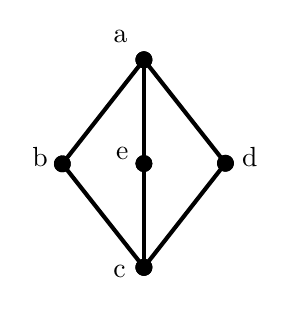
\begin{tikzpicture}[x=0.75pt,y=0.75pt,yscale=-1,xscale=1]
        \path (0,131); %set diagram left start at 0, and has height of 131
        %Straight Lines [id:da15970001891170416] 
        \draw [line width=1.5]    (56,17) -- (56,67) ;
        \draw [shift={(56,67)}, rotate = 90] [color={rgb, 255:red, 0; green, 0; blue, 0 }  ][fill={rgb, 255:red, 0; green, 0; blue, 0 }  ][line width=1.5]      (0, 0) circle [x radius= 3.05, y radius= 3.05]   ;
        \draw [shift={(56,17)}, rotate = 90] [color={rgb, 255:red, 0; green, 0; blue, 0 }  ][fill={rgb, 255:red, 0; green, 0; blue, 0 }  ][line width=1.5]      (0, 0) circle [x radius= 3.05, y radius= 3.05]   ;
        %Straight Lines [id:da08966008188804464] 
        \draw [line width=1.5]    (56,67) -- (56,117) ;
        \draw [shift={(56,117)}, rotate = 90] [color={rgb, 255:red, 0; green, 0; blue, 0 }  ][fill={rgb, 255:red, 0; green, 0; blue, 0 }  ][line width=1.5]      (0, 0) circle [x radius= 3.05, y radius= 3.05]   ;
        \draw [shift={(56,67)}, rotate = 90] [color={rgb, 255:red, 0; green, 0; blue, 0 }  ][fill={rgb, 255:red, 0; green, 0; blue, 0 }  ][line width=1.5]      (0, 0) circle [x radius= 3.05, y radius= 3.05]   ;
        %Straight Lines [id:da9950631870470763] 
        \draw [line width=1.5]    (56,17) -- (95.29,66.86) ;
        \draw [shift={(95.29,66.86)}, rotate = 51.76] [color={rgb, 255:red, 0; green, 0; blue, 0 }  ][fill={rgb, 255:red, 0; green, 0; blue, 0 }  ][line width=1.5]      (0, 0) circle [x radius= 3.05, y radius= 3.05]   ;
        \draw [shift={(56,17)}, rotate = 51.76] [color={rgb, 255:red, 0; green, 0; blue, 0 }  ][fill={rgb, 255:red, 0; green, 0; blue, 0 }  ][line width=1.5]      (0, 0) circle [x radius= 3.05, y radius= 3.05]   ;
        %Straight Lines [id:da1687670314559928] 
        \draw [line width=1.5]    (56,117) -- (95.29,66.86) ;
        \draw [shift={(95.29,66.86)}, rotate = 308.08] [color={rgb, 255:red, 0; green, 0; blue, 0 }  ][fill={rgb, 255:red, 0; green, 0; blue, 0 }  ][line width=1.5]      (0, 0) circle [x radius= 3.05, y radius= 3.05]   ;
        \draw [shift={(56,117)}, rotate = 308.08] [color={rgb, 255:red, 0; green, 0; blue, 0 }  ][fill={rgb, 255:red, 0; green, 0; blue, 0 }  ][line width=1.5]      (0, 0) circle [x radius= 3.05, y radius= 3.05]   ;
        %Straight Lines [id:da19938433470927985] 
        \draw [line width=1.5]    (16.71,67.14) -- (56,117) ;
        \draw [shift={(56,117)}, rotate = 51.76] [color={rgb, 255:red, 0; green, 0; blue, 0 }  ][fill={rgb, 255:red, 0; green, 0; blue, 0 }  ][line width=1.5]      (0, 0) circle [x radius= 3.05, y radius= 3.05]   ;
        \draw [shift={(16.71,67.14)}, rotate = 51.76] [color={rgb, 255:red, 0; green, 0; blue, 0 }  ][fill={rgb, 255:red, 0; green, 0; blue, 0 }  ][line width=1.5]      (0, 0) circle [x radius= 3.05, y radius= 3.05]   ;
        %Straight Lines [id:da7933561944435159] 
        \draw [line width=1.5]    (56,17) -- (16.71,67.14) ;
        \draw [shift={(16.71,67.14)}, rotate = 128.08] [color={rgb, 255:red, 0; green, 0; blue, 0 }  ][fill={rgb, 255:red, 0; green, 0; blue, 0 }  ][line width=1.5]      (0, 0) circle [x radius= 3.05, y radius= 3.05]   ;
        \draw [shift={(56,17)}, rotate = 128.08] [color={rgb, 255:red, 0; green, 0; blue, 0 }  ][fill={rgb, 255:red, 0; green, 0; blue, 0 }  ][line width=1.5]      (0, 0) circle [x radius= 3.05, y radius= 3.05]   ;

        % Text Node
        \draw (40,1.8) node [anchor=north west][inner sep=0.75pt]   [align=left] {a};
        % Text Node
        \draw (1,57.8) node [anchor=north west][inner sep=0.75pt]   [align=left] {b};
        % Text Node
        \draw (102,57.8) node [anchor=north west][inner sep=0.75pt]   [align=left] {d};
        % Text Node
        \draw (41.33,57.8) node [anchor=north west][inner sep=0.75pt]   [align=left] {e};
        % Text Node
        \draw (40,114.8) node [anchor=north west][inner sep=0.75pt]   [align=left] {c};
        \end{tikzpicture}}
    \end{wrapfigure}
    Prove that Diamond is not a distributive lattice:
    \begin{definition}{(Distributivity)}{}
        A lattice with the following properties:
        \useshortskip
        \[
            \begin{array}{c}
                x \wedge (y \vee z) = (x \wedge y) \vee (x \wedge z)  \\
                x \vee (y \wedge z) = (x \vee y) \wedge (x \vee z)              
            \end{array}
        \]
        is called distributive.
    \end{definition}
\end{problem}
\begin{solution}
    The property does not hold for elements, e.g. $b, e, d$:
    \[
        \begin{array}{c}
            \displaystyle b \wedge (e \vee d) = b \wedge a = b  \\[0.1cm]
            \resizebox{8pt}{14pt}{\rotatebox{90}{\neq}}\\
            \displaystyle (b \wedge e) \vee (e \wedge d) = c \vee c = c            
        \end{array}
    \]
\end{solution}
\vspace*{-1.5cm}

\begin{problem}{}
    Take 5 last banks from slide 3 – Rotschild, Santander, SG, UBP, UBS – as objects and 7 bank properties –BankType:Investment, BankType:Private, BankType:Universal, Owner:Private, Owner:Public, Code:Explicit, Code:No – as binary attributes. Compose the formal context with 5 objects (banks),  7 attributes (bank properties), and incidence relation according to the table in slide 3. Manually compute all concepts of this context, construct the diagram of the concept lattice and give three valid implications ofthis context.
\begin{figure}[h!]  
    \centering  
    \begin{tabular}{llllllllll}
        \hline
        Case                            & Country & BankType   & Owner   & Code     & CorpC & FinLib & RegInt & BList & Wolfs                    \\ \hline
        \multicolumn{1}{|l}{Rothschild} & GBR     & Investment & Private & No       & 0.14  & 1      & 277    & Yes   & \multicolumn{1}{l|}{No}  \\
        \multicolumn{1}{|l}{Santander}  & ESP     & Universal  & Public  & Explicit & 0.77  & 1      & 53     & No    & \multicolumn{1}{l|}{Yes} \\
        \multicolumn{1}{|l}{SG}         & FRA     & Universal  & Public  & Explicit & 0.82  & 1      & 75     & No    & \multicolumn{1}{l|}{Yes} \\
        \multicolumn{1}{|l}{UBP}        & CHE     & Private    & Private & No       & 0.44  & 0.95   & 83     & Yes   & \multicolumn{1}{l|}{No}  \\
        \multicolumn{1}{|l}{UBS}        & CHE     & Universal  & Public  & Explicit & 0.44  & 0.95   & 83     & Yes   & \multicolumn{1}{l|}{Yes} \\ \hline
        \end{tabular}
\end{figure}
\end{problem}
\begin{solution}
    Let's start with building objects-attributes table:
    \begin{figure}[h!]
        \centering 
        \begin{tabular}{|l|c|lllllll|c|}
            \hline
              & \multicolumn{1}{l|}{\diagbox[width=6em]{G}{M}} & \multicolumn{1}{c}{a} & \multicolumn{1}{c}{b} & \multicolumn{1}{c}{c} & \multicolumn{1}{c}{d} & \multicolumn{1}{c}{e} & \multicolumn{1}{c}{f} & \multicolumn{1}{c|}{g} & \multicolumn{1}{l|}{Wolf} \\ \hline
            1 & Rothschild                                                  & $\times$              &                       &                       & $\times$              &                       &                       & $\times$               & -                         \\
            2 & Santander                                                   &                       & $\times$              &                       &                       & $\times$              & $\times$              &                        & +                         \\
            3 & SG                                                          &                       & $\times$              &                       &                       & $\times$              & $\times$              &                        & +                         \\
            4 & UBP                                                         &                       &                       & $\times$              & $\times$              &                       &                       & $\times$               & -                         \\
            5 & UBS                                                         &                       & $\times$              &                       &                       & $\times$              & $\times$              &                        & +                         \\ \hline
            \end{tabular}
    \end{figure}
    \begin{center}
        {\large Attributes}        
    \end{center}
\begin{multicols}{3}
    \begin{itemize}
        \item[{\large a --}] BankType: Investment; 
        \item[{\large b --}] BankType: Universal;
        \item[{\large c --}] BankType: Private;
        \item[{\large d --}] Owner: Private;
        \item[{\large e --}] Owner: Public;
        \item[{\large f --}] Code: Explicit;
        \item[{\large g --}] Code: No.
    \end{itemize}
    {\large Objects:} banks
\end{multicols}
\begin{figure}[h!]
    \centering
    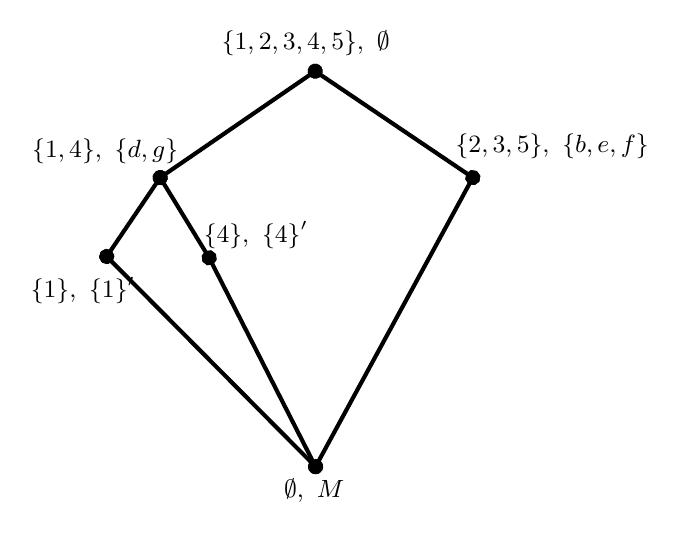
\begin{tikzpicture}[x=0.75pt,y=0.75pt,yscale=-1,xscale=1]
        %uncomment if require: \path (0,244); %set diagram left start at 0, and has height of 244
        
        %Straight Lines [id:da3418589839093764] 
        \draw [line width=1.5]    (139.59,31) -- (215.53,82.26) ;
        \draw [shift={(215.53,82.26)}, rotate = 34.02] [color={rgb, 255:red, 0; green, 0; blue, 0 }  ][fill={rgb, 255:red, 0; green, 0; blue, 0 }  ][line width=1.5]      (0, 0) circle [x radius= 2.61, y radius= 2.61]   ;
        \draw [shift={(139.59,31)}, rotate = 34.02] [color={rgb, 255:red, 0; green, 0; blue, 0 }  ][fill={rgb, 255:red, 0; green, 0; blue, 0 }  ][line width=1.5]      (0, 0) circle [x radius= 2.61, y radius= 2.61]   ;
        %Straight Lines [id:da0861135406925968] 
        \draw [line width=1.5]    (64.91,82.26) -- (139.59,31) ;
        \draw [shift={(139.59,31)}, rotate = 325.53] [color={rgb, 255:red, 0; green, 0; blue, 0 }  ][fill={rgb, 255:red, 0; green, 0; blue, 0 }  ][line width=1.5]      (0, 0) circle [x radius= 2.61, y radius= 2.61]   ;
        \draw [shift={(64.91,82.26)}, rotate = 325.53] [color={rgb, 255:red, 0; green, 0; blue, 0 }  ][fill={rgb, 255:red, 0; green, 0; blue, 0 }  ][line width=1.5]      (0, 0) circle [x radius= 2.61, y radius= 2.61]   ;
        %Straight Lines [id:da8536312806368171] 
        \draw [line width=1.5]    (64.91,82.26) -- (39.14,120.28) ;
        \draw [shift={(39.14,120.28)}, rotate = 124.13] [color={rgb, 255:red, 0; green, 0; blue, 0 }  ][fill={rgb, 255:red, 0; green, 0; blue, 0 }  ][line width=1.5]      (0, 0) circle [x radius= 2.61, y radius= 2.61]   ;
        \draw [shift={(64.91,82.26)}, rotate = 124.13] [color={rgb, 255:red, 0; green, 0; blue, 0 }  ][fill={rgb, 255:red, 0; green, 0; blue, 0 }  ][line width=1.5]      (0, 0) circle [x radius= 2.61, y radius= 2.61]   ;
        %Straight Lines [id:da43109469886366125] 
        \draw [line width=1.5]    (64.91,82.26) -- (88.51,120.91) ;
        \draw [shift={(88.51,120.91)}, rotate = 58.59] [color={rgb, 255:red, 0; green, 0; blue, 0 }  ][fill={rgb, 255:red, 0; green, 0; blue, 0 }  ][line width=1.5]      (0, 0) circle [x radius= 2.61, y radius= 2.61]   ;
        \draw [shift={(64.91,82.26)}, rotate = 58.59] [color={rgb, 255:red, 0; green, 0; blue, 0 }  ][fill={rgb, 255:red, 0; green, 0; blue, 0 }  ][line width=1.5]      (0, 0) circle [x radius= 2.61, y radius= 2.61]   ;
        %Straight Lines [id:da6107845838444239] 
        \draw [line width=1.5]    (215.53,82.26) -- (139.77,221.54) ;
        \draw [shift={(139.77,221.54)}, rotate = 118.55] [color={rgb, 255:red, 0; green, 0; blue, 0 }  ][fill={rgb, 255:red, 0; green, 0; blue, 0 }  ][line width=1.5]      (0, 0) circle [x radius= 2.61, y radius= 2.61]   ;
        \draw [shift={(215.53,82.26)}, rotate = 118.55] [color={rgb, 255:red, 0; green, 0; blue, 0 }  ][fill={rgb, 255:red, 0; green, 0; blue, 0 }  ][line width=1.5]      (0, 0) circle [x radius= 2.61, y radius= 2.61]   ;
        %Straight Lines [id:da7447679180659528] 
        \draw [line width=1.5]    (39.14,120.28) -- (139.77,221.54) ;
        \draw [shift={(139.77,221.54)}, rotate = 45.18] [color={rgb, 255:red, 0; green, 0; blue, 0 }  ][fill={rgb, 255:red, 0; green, 0; blue, 0 }  ][line width=1.5]      (0, 0) circle [x radius= 2.61, y radius= 2.61]   ;
        \draw [shift={(39.14,120.28)}, rotate = 45.18] [color={rgb, 255:red, 0; green, 0; blue, 0 }  ][fill={rgb, 255:red, 0; green, 0; blue, 0 }  ][line width=1.5]      (0, 0) circle [x radius= 2.61, y radius= 2.61]   ;
        %Straight Lines [id:da33697907813025085] 
        \draw [line width=1.5]    (88.51,120.91) -- (139.77,221.54) ;
        \draw [shift={(139.77,221.54)}, rotate = 63] [color={rgb, 255:red, 0; green, 0; blue, 0 }  ][fill={rgb, 255:red, 0; green, 0; blue, 0 }  ][line width=1.5]      (0, 0) circle [x radius= 2.61, y radius= 2.61]   ;
        \draw [shift={(88.51,120.91)}, rotate = 63] [color={rgb, 255:red, 0; green, 0; blue, 0 }  ][fill={rgb, 255:red, 0; green, 0; blue, 0 }  ][line width=1.5]      (0, 0) circle [x radius= 2.61, y radius= 2.61]   ;
        
        % Text Node
        \draw (93.33,10.3) node [anchor=north west][inner sep=0.75pt]  [font=\small] [align=left] {$\displaystyle \{1,2,3,4,5\} ,\ \emptyset $};
        % Text Node
        \draw (206,60.13) node [anchor=north west][inner sep=0.75pt]  [font=\small] [align=left] {$\displaystyle \{2,3,5\} ,\ \{b,e,f\}$};
        % Text Node
        \draw (2,62.13) node [anchor=north west][inner sep=0.75pt]  [font=\small] [align=left] {$\displaystyle \{1,4\} ,\ \{d,g\}$};
        % Text Node
        \draw (1.33,128.8) node [anchor=north west][inner sep=0.75pt]  [font=\small] [align=left] {$\displaystyle \{1\} ,\ \{1\} '$};
        % Text Node
        \draw (84.67,102.13) node [anchor=north west][inner sep=0.75pt]  [font=\small] [align=left] {$\displaystyle \{4\} ,\ \{4\} '$};
        % Text Node
        \draw (123.33,226.13) node [anchor=north west][inner sep=0.75pt]  [font=\small] [align=left] {$\displaystyle \emptyset ,\ M$};
        \end{tikzpicture}               
\end{figure}

Implications:
\[
  \begin{array}{c}
    abc \to d\\
    a \to d\\
    cg \to a
  \end{array}  
\]
\end{solution}

\begin{problem}{}
    Choose your option for the big homework.
\end{problem}
\begin{solution}
    I want to select Lazy FCA option as my big homework.
\end{solution}
\end{document}